%%%%%%%%%% PREAMBLE %%%%%%%%%%%%%%

\documentclass[xcolor=pdftex,dvipsnames,table]{beamer}

\usepackage[utf8]{inputenc}
\usepackage[english]{babel}

\usepackage{minted}
\usepackage{transparent}
\usepackage{multimedia}
\usepackage{tcolorbox}

\graphicspath{{./figures/}}

\definecolor{bgConsole}{HTML}{ffffcc}

%%%%%%%%%% THEME %%%%%%%%%%%%%%

\mode<presentation>
{
  \usetheme{Madrid}
  \usecolortheme{seagull}
  \setbeamercovered{dynamic} %invisible,transparent,dynamic,highly dynamic
}

%%%%%%%%%% COVER %%%%%%%%%%%%%%%

\title{Floorplan Design of VLSI Circuits}

\author[A. Abella]{Arnau ~Abella\inst{1}}

\institute[UPC]
{
  \inst{1}%
  Universitat Polit\`ecnica de Barcelona
}

\date{\today}

% \logo{\includegraphics[height=0.5cm]{haskell-logo.png}}

%%%%%%%%%% FRAMES %%%%%%%%%%%%%%%

\AtBeginSection[]
{
  \begin{frame}<beamer>
      \frametitle{Table of Contents}
      \tableofcontents[currentsection]
  \end{frame}
}

\begin{document}

% Cover
\frame{\titlepage}

% Intro
\section{Introduction}
\begin{frame}{Introduction}
  \begin{block}{Floorplan design}<1->
    It is the problem of placing a given set of circuits modules in the plane to minimize
    a weighted sum of the following two quantities:
    \begin{itemize}
      \item the \textbf{area} of the bounding rectangle containing all the modules
      \item an estimation of the total interconnection \textbf{wire length}
    \end{itemize}
  \end{block}
  \begin{block}{Module}<2>
    A module can be classified as:
    \begin{itemize}
      \item \textbf{rigid}, if its shape and dimensions are rigid (e.g. library macrocells)
      \item \textbf{flexible}, if its shape and dimensions are not fixed (assume rectangular modules)
    \end{itemize}
  \end{block}
\end{frame}

\begin{frame}[allowframebreaks]{Floorplan}
  \begin{block}{}
    A \textbf{floorplan} for $n$ given modules (named $1,2,\ldots,n$) consist of an enveloping rectangle $R$
    subdivided by horizontal and vertical line segments into $n$ or more nonoverlapping rectilinear regions.
  \end{block}
  \begin{block}{}
    The \textbf{aspect ratio} of $R$ must be between two given numbers $p$ and $q$.
  \end{block}
  \begin{block}{}
    We are given an $n \times n$ \textbf{interconnection matrix } $C = (c_{ij})_{n \times n}$ with $c_{ij} \geq 0, 1 \leq i,j \leq n$ which provides information on the wiring density between each pair of modules. The \textit{distance} between two regions is the Manhattan distance between their centers. For every pair of modules $i$ and $j$, let $d_{ij}$ be the distance between regions $i$ and $j$.
  \end{block}
  \begin{block}{}
    Let $A$ be the area of $R$.
    \newline

    We use $W = \sum_{1 \leq i,j \leq n} c_{ij}d_{ij}$ as an estimate of the total interconnection wire length.
    \newline

    We use $A + \lambda W$ to measure the \textbf{quality} of the floorplan, where $\lambda$ is a user-specified constant.
  \end{block}
\end{frame}

% Algorithm
\section{Algorithm}

\begin{frame}{The original work}
  \begin{block}{}
    This work is based on \textit{"Floorplan Design of VLSI Circuits"} \cite{Wong1989}.
  \end{block}
  \begin{block}{}
    The algorithm uses \textbf{Polish expressions} to represent floorplans and employ a search method
    called \textbf{simulated annealing} \cite{Ki1983}. The final solution is derived in two stages:
    \begin{itemize}
      \pause
      \item first determine the relative positions of the modules using primarily interconnection information,
      \pause
      \item then, use the area and shape information to minimize the area of the bounding rectangle
    \end{itemize}
  \end{block}
\end{frame}

\begin{frame}[allowframebreaks]{Rectangular Modules}
  \begin{block}{Rectangular floorplan}
    A \textit{rectangular floorplan} is a floorplan where all the regions are rectangles.
  \end{block}

  We shall only consider rectangular floorplans.

  \begin{block}{}
    Let $(A_1, r_1, s_1),(A_2, r_2, s_2),\ldots,(A_n, r_n, s_n)$ be a list of $n$ triplets of numbers corresponding to the $n$ given modules. The triplet of numbers $(A_i, r_i, s_i)$, with $r_i \leq s_i$, specifies the area and the limits of the allowed aspect ratio for module $i$.
  \end{block}

  \begin{block}{}
    Each module can also have a \textit{fixed} or \textit{free} orientation (90$^\circ$ rotations are allowed). Let $O_1$ be the set of modules with fixed orientation, and $O_2$ be the set of modules with free orientation. Let $w_i$ be the width and $h_i$ be the height of module $i$, we must have:

    \begin{align}
      &w_ih_i = A_i\\
      &r_i \leq h_i/w_i \leq s_i &\text{if } i \in O_1\\
      &r_i \leq h_i/w_i \leq s_i \text{ or } 1/s_i \leq h_i/w_i \leq 1/r_i &\text{if } i \in O_2
    \end{align}
  \end{block}
\end{frame}

\begin{frame}{Slicing Floorplans}
  \begin{block}{Slicing floorplan}
    A \textit{slicing floorplan} is a rectangular floorplan with $n$ basic rectangles that can be obtained by recursively cutting a rectangle into smaller rectangles (see Figure \ref{fig:1}(a)). It can be represented by an oriented rooted binary tree, called \textit{slicing tree} (see Figure \ref{fig:1}(b)).
  \end{block}
  \begin{figure}
    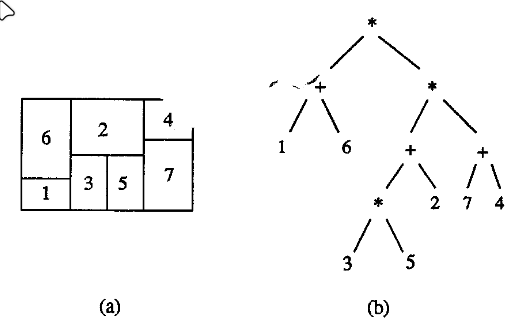
\includegraphics[trim={0 0 0 0.5cm}, scale=0.3, clip]{slicing_floorplan}
    \caption{Slicing floorplan and its slicing tree representation.}
    \label{fig:1}
  \end{figure}
\end{frame}

\begin{frame}{Slicing Floorplans}
  No dimensional information is given by a slicing tree.
  Note that for a given slicing floorplan, there may be more than one slicing-tree representation.
  \begin{block}{Slicing Structure}
    Let $A$ and $B$ be two slicing floorplans. We define $A \sim B$ iff they have the same slicing tree representation. The equivalence relation $\sim$ partitions the set of slicing floorplans into equivalence classes. Each equivalence class of slicing floorplans with $n$ basic rectangles is called a \textbf{slicing structure}.
  \end{block}
\end{frame}

\begin{frame}{Slicing Floorplans}
  \begin{block}{Skewed slicing tree}
    A \textit{skewed slicing tree} is a slicing tree in which no node and its right son have the same label in $\{*,+\}$ (see Figure \ref{fig:2}).
  \end{block}

  \begin{figure}
    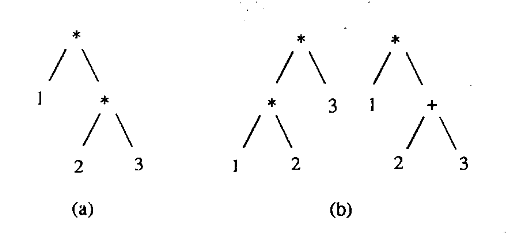
\includegraphics[scale=0.5]{skewed_tree}
    \caption{(a) A nonskewed slicing tree; (b) skewed slicing tree.}
    \label{fig:2}
  \end{figure}
\end{frame}

\begin{frame}{Solution Space}
  \begin{lemma}\label{lemma:1}
    There is a $1-1$ correspondence between all skewed slicing trees with $n$ leaves and all slicing structures with $n$ basic rectangles.
  \end{lemma}

  Instead of using the set of all slicing floorplans as the solution space, we can use the set of all slicing structures as the solution space. This \textbf{substantially reduces} the size of the solution space.
\end{frame}

\begin{frame}{Solution Space}
  \begin{block}{Polish expression}
    We use a representation of slicing structures called \textbf{normalized Polish expressions} that are particularly suitable for the method of simulated annealing.
  \end{block}

  \begin{lemma}\label{lemma:2}
    There is a $1-1$ correspondence between the set of normalized Polish expressions of length $2n - 1$  and the set of skewed slicing trees with $n$ leaves.
  \end{lemma}
\end{frame}

\begin{frame}{Solution Space}
  \begin{theorem}\label{theorem:1}
    There is a $1-1$  correspondence between the set of normalized Polish expressions of length $2n-1$ and the set of slicing structures with $n$ basic rectangles.
  \end{theorem}

  We use the set of normalized Polish expressions as the \textbf{solution space}.
\end{frame}

\begin{frame}{Polish Expression}
  \begin{block}{}
    Let $\alpha = \alpha_1 \alpha_2 \cdots \alpha_{2n-1}$ be a normalized Polish expression. Note that $\alpha$ can also be written as $c_0 \pi_1 c_2 \pi_2 c_2 \cdots c_{n-1} \pi_n c_n$, where $\pi_1, \pi_2, \ldots, \pi_n$ is a permutation of $1,2,\ldots, n$, the $c_i$'s are chains. and $\sum_i l(c_i) = n - 1$.
  \end{block}

  \begin{figure}
    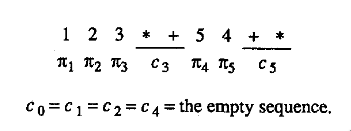
\includegraphics[scale=0.5]{polish_expression}
    \caption{Chains in a Polish expression.}
    \label{fig:3}
  \end{figure}
\end{frame}

\begin{frame}{Polish Expression}
  \begin{block}{}
    Two operands in $\alpha$ are said to be \textit{adjacent} iff they are consecutive elements in $\pi_1 \cdots \pi_n$. An operand and operator are said to be \textit{adjacent} iff they are consecutives elements in $\alpha_1 \alpha_2 \cdots \alpha_{2n-1}$.
  \end{block}
  We define three types of moves, $M1, M2, \text{and } M3$, that can be used to modify a given normalized Polish expression (see Figure \ref{fig:3}):
  \begin{itemize}
      \pause
      \item $M1$. Swap two adjacent operands.
      \pause
      \item $M2$. Complement a chain of nonzero length.
      \pause
      \item $M3$. Swap two adjacent operand and operator.
  \end{itemize}
\end{frame}

\begin{frame}{Polish Expression}
  \begin{figure}
    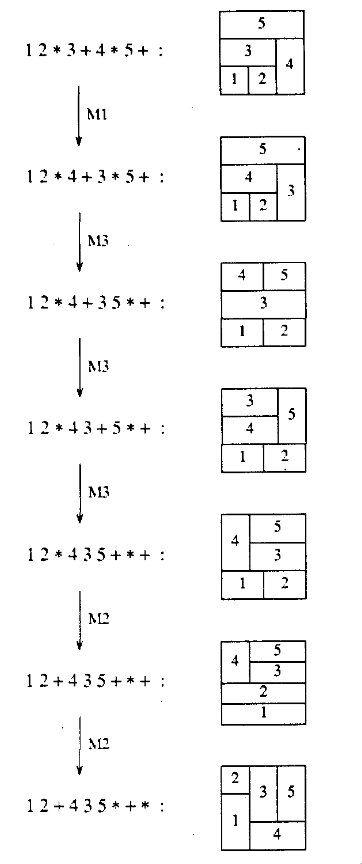
\includegraphics[scale=0.3]{moves}
    \caption{Illustration of the moves.}
    \label{fig:4}
  \end{figure}
\end{frame}

\begin{frame}{Cost Function}
  \begin{block}{}
    Let $\alpha$ be a normalized Polish expression. The expression $\alpha$ represents a set $S_\alpha$ of equivalent slicing floorplans. Let $f_\alpha$ be a floorplan in $S_\alpha$ with minimum area. Let $A(\alpha)$ and $W(\alpha)$ be the area and the total wirelength of $f_\alpha$, respectively. The cost function we use is $\Psi(\alpha) = A(\alpha) + \lambda W(\alpha)$.
  \end{block}

  We can efficiently compute $\Psi(\alpha)$ for a given normalized Polish expression $\alpha$.
\end{frame}

\begin{frame}{Cost Function}
  \begin{definition}
    Let $\Gamma$ be a continuous curve on the plane. $\Gamma$ is a \textbf{shape curve} if it satisfies the following conditions:
  \begin{enumerate}
    \item It is decreasing and lies completely in the first quadrant
    \item $\exists k > 0$ such that all lines of the form $x = a, a > k$, intersect $\Gamma$, and
    \item $\exists k > 0$ such that all lines of the form $y = b, b > k$, intersect $\Gamma$.
  \end{enumerate}
  \end{definition}
  \begin{definition}
    Let $\Gamma$ and $\Lambda$ be two shape curves. We define $\Gamma + \Lambda$ to be the curve $\{(u, v+w)| (u,v) \in \Gamma \text{ and } (u, w) \in \Lambda\}$ and define $\Gamma * \Lambda$ to be the curve $\{(u+v, w)| (u,w) \in \Gamma \text{ and } (v, w) \in \Lambda\}$. It is easy to see that $\Gamma + \Lambda$ and $\Gamma * \Lambda$ are also shape curves.
  \end{definition}
\end{frame}

\begin{frame}{Cost Function}
  \begin{definition}
  \end{definition}
  \begin{figure}
    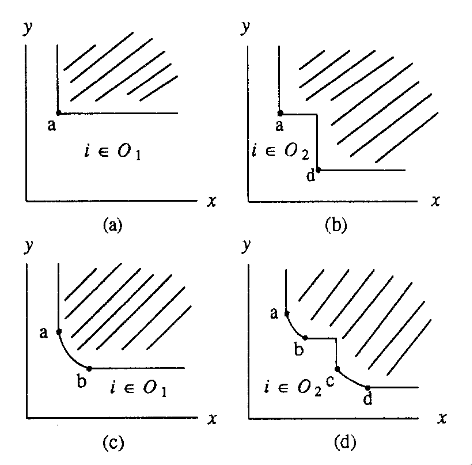
\includegraphics[scale=0.4]{shape_curves}
    \caption{Shape curves for different shape constraints.}
    \label{fig:5}
  \end{figure}
\end{frame}

\begin{frame}{Cost Function}
  \begin{block}{Area Computation}
    Let $T_\alpha$ be the slicing tree corresponding to $\alpha$. For each node $v$ in $T_\alpha$, the subtree rooted at $v$ defines a slicing structure $R_v$. Let $\Gamma_v$ be the shape curve representing the shape constraints for $R_v$.
    \newline

    \pause
    For every three node $u,v, w$ in $T_\alpha$ with $v$ being the father of $u$ and $w$, $\Gamma_v$ is either $\Gamma_u * \Gamma_w$ or $\Gamma_u + \Gamma_w$ depending on whether $v$ is $*$ or $+$.
    \newline

    \pause
    Once we have computed all the $\Gamma_v$'s, we can compute the area measure $A(\alpha)$ from $\Gamma_r$ where $r$ is the root of the $T_\alpha$.
  \end{block}
\end{frame}

\begin{frame}{Cost Function}
  \begin{block}{Wire Length Computation}
    Since $T_\alpha$ is a slicing tree representation of $f_\alpha$, each node $v$ in $T_\alpha$ corresponds to a rectangle $K_v$ in $f_\alpha$. Let $(x_v, y_v)$ be the dimensions of $K_v$. After we have computed $(x_r, y_r)$ for $K_r$ where $r$ is the root of $T_\alpha$, we can recursively compute the dimensions of all the basic rectangles \mbox{(see \cite{Wong1989})}.
    \newline
    \pause

    Let $(C_v^x, C_v^y)$ be the coordinates of the center of $K_v$. It follows that the $d_{ij}$'s (the distances between the basic rectangles) and consequently $W(\alpha)$ can be easily computed from the $(c_v^x, c_v^y)$'s.
  \end{block}
\end{frame}

\begin{frame}{Cost Function}
  \begin{block}{Incremental Computation of Cost Function}
    For a given normalized Polish expression, the shape curves associating with the nodes of its slicing tree are needed in both the area and wire length computation.
    \newline

    \pause
    In our simulated annealing algorithm, each move leads to only a minor modification of the Polish expression currently being examined.
    \newline

    \pause
    Let $\alpha' = \alpha'_1 \alpha'_2 \cdots \alpha'_{2n-1}$ be the Polish expression obtained from $\alpha = \alpha_1 \alpha_2 \cdots \alpha_{2n-1}$ after a move. In general, $\Gamma_i = \Gamma'_i$ for many $i$'s. Therefore, in computing the cost for $\alpha'$, we need only update those shape curves that are changed.
  \end{block}
\end{frame}

\begin{frame}{Cost Function}
  \begin{theorem}\label{theorem:2}
    Let $\alpha'$ be the Polish expression obtained from $\alpha$ after a move. The shape curves $\Gamma_i$'s and the shape curves $\Gamma'_i$'s differ only at a set of vertices that lie along one or two path in each of $T_\alpha$ and $T_{\alpha'}$
  \end{theorem}

  Figure \ref{fig:6} illustrates the statement in Theorem \ref{theorem:2}.
\end{frame}

\begin{frame}{Cost Function}
  \begin{figure}
    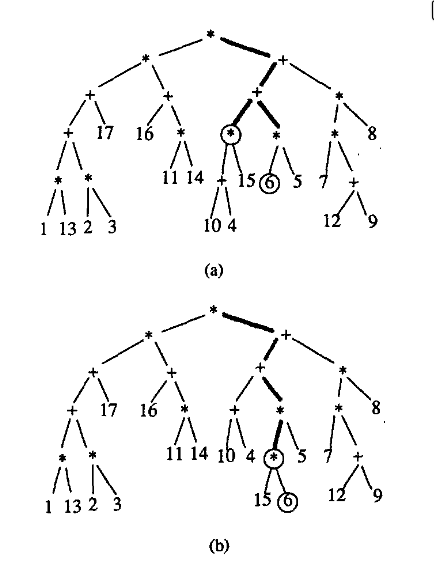
\includegraphics[scale=0.4]{incremental_computation}
    \caption{The path(s) in $T_\alpha$ and $T_{\alpha'}$ after a move.}
    \label{fig:6}
  \end{figure}
\end{frame}

% Implementation
\section{Implementation}

\begin{frame}{Implementation}
  \begin{block}{}
    The algorithm is implemented in \textit{haskell} (compiler \textit{GHC 8.8.4}).
    The executable can be build using \textit{cabal}, \textit{stack} or \textit{nix}.
  \end{block}
  \begin{block}{}
    Apart from the algorithm, there is also a command-line interface executable with a custom problem file format with its corresponding parser.
    The executable allows to generate random instances for testing.
  \end{block}
  \begin{block}{}
    The code is public and available at \url{https://github.com/monadplus/floorplanning}.
  \end{block}
\end{frame}

\begin{frame}{Implementation}
  \begin{itemize}
      \item app/
        \begin{itemize}
          \item Main.hs (111 lines)
        \end{itemize}
      \item src/
        \begin{itemize}
          \item Floorplan.hs (51 lines)
            \item Floorplan/
              \begin{itemize}
                \item PolishExpression.hs (376 lines)
                \item Pretty.hs (61 lines)
                \item Problem.hs (226)
                \item Report.hs (51 lines)
                \item SimulatedAnnealing.hs (590 lines)
                \item SlicingTree.hs (56 lines)
                \item Types.hs (174 lines)
              \end{itemize}
        \end{itemize}
      \item test/
        \begin{itemize}
          \item Spec.hs (22 lines)
            \item Test/
              \begin{itemize}
                \item PolishExpression.hs (121 lines)
                \item Pretty.hs (77 lines)
                \item Problem.hs (57 lines)
                \item SimulatedAnnealing.hs (326 lines)
              \end{itemize}
        \end{itemize}
  \end{itemize}
\end{frame}

%\begin{frame}[fragile, t]{Implementation}
  %\begin{listing}[ht]
  %\begin{minted}[bgcolor=bg, fontsize=\footnotesize, escapeinside=||]{haskell}

  %\end{minted}
    %\caption{}
  %\label{listing:1}
  %\end{listing}
%\end{frame}

% Results
\section{Results}

\begin{frame}{Results}
  \begin{table}[]
  \begin{tabular}{cccccc}
          &      &             &            & \multicolumn{2}{c}{Final solution} \\ \cline{5-6}
  Problem & $n$  & $\lambda_w$ & $A_{min}$  & $A$              & $W$             \\ \hline
     P1   & $10$ & $0.5$       & $33.0$     & $35.0$           & $53.0$          \\
     P1   & $10$ & $1.0$       & $33.0$     & $35.0$           & $46.0$          \\
     P2   & $15$ & $0.5$       & $144.0$    & $153.0$          & $179.5$         \\
     P3   & $20$ & $0.5$       & $92.0$     & $108.0$          & $151.5$         \\
     P3   & $20$ & $1.0$       & $92.0$     & $117.0$          & $118.5$         \\
     P4   & $30$ & $0.5$       & $199.0$    & $231.0$          & $1037.5$        \\
     P5   & $40$ & $1.0$       & $325.0$    & $400.0$          & $1895.5$        \\
     P6   & $50$ & $1.0$       & $445.0$    & $529.0$          & $4150.0$        \\
  \end{tabular}
  \caption{Experimental results}
  \end{table}
\end{frame}

% Demo
\section{Demo}

%\begin{frame}{Demo}
  %% FIXME https://github.com/andersx/beamer-gif
  %\movie[loop,width=\textwidth]{
    %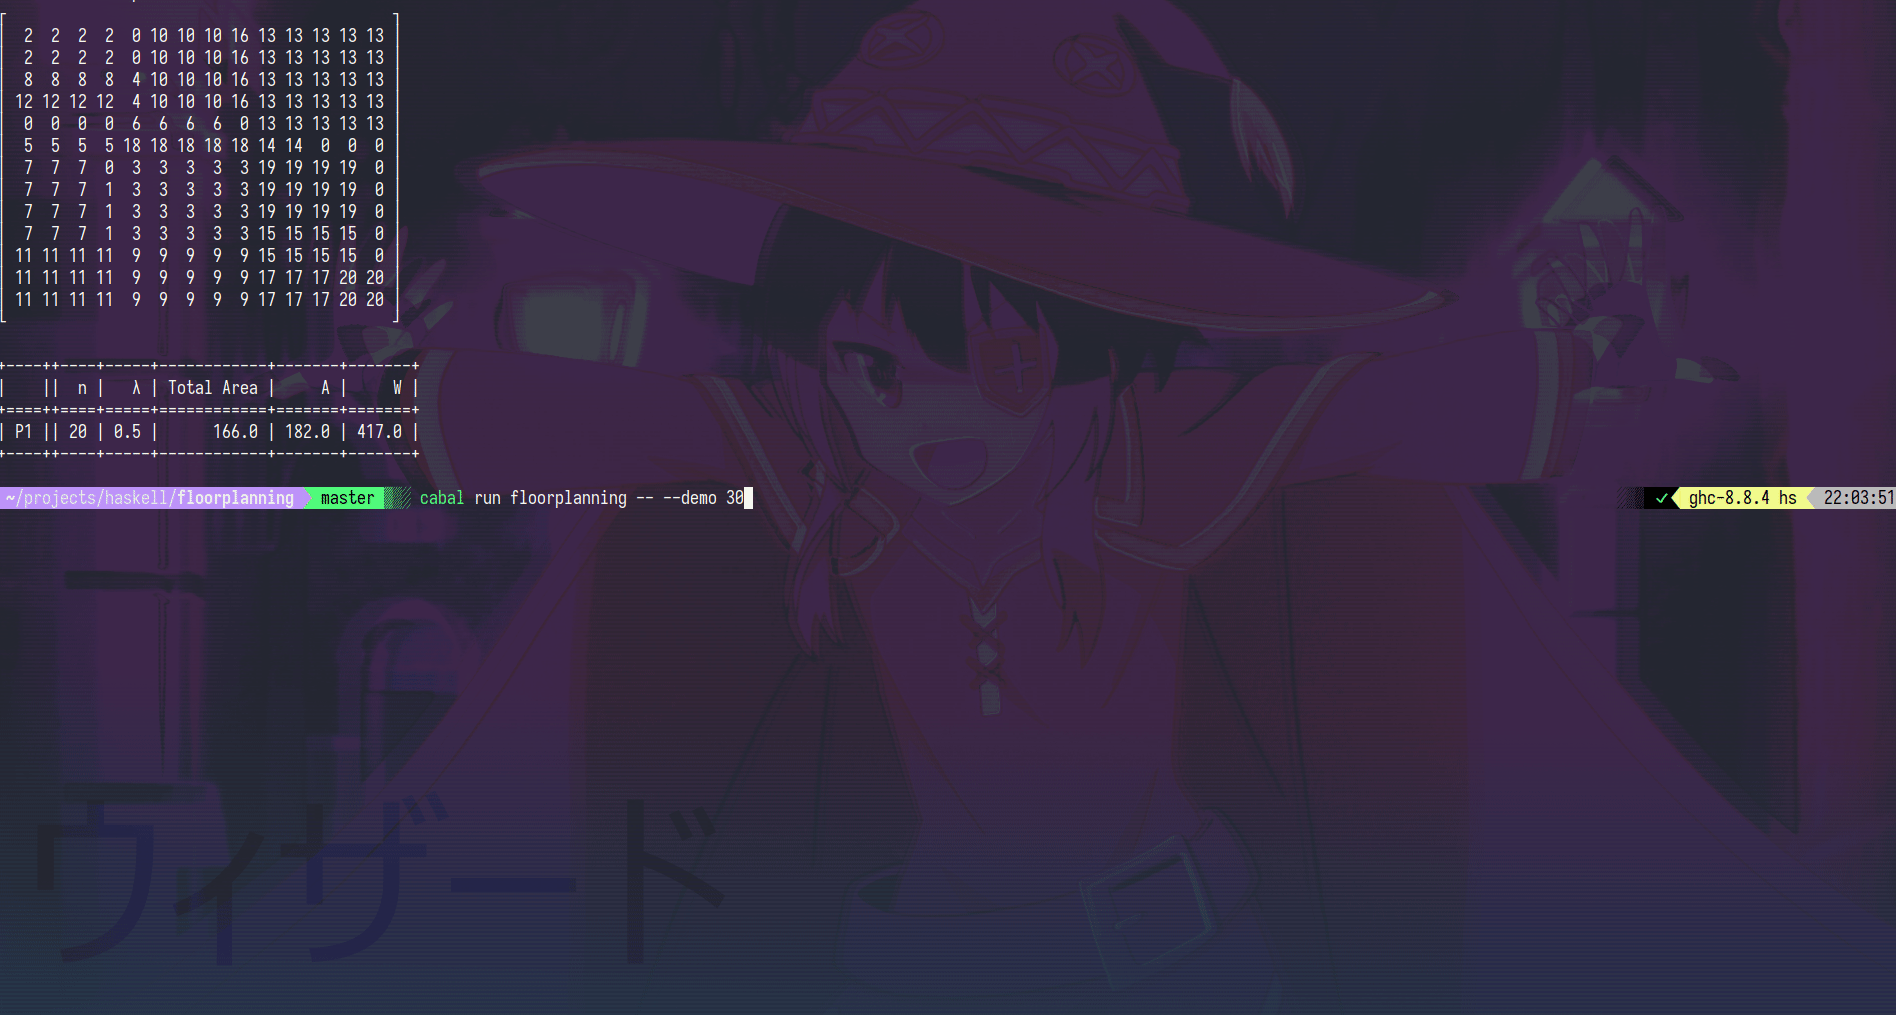
\includegraphics[width=\textwidth]{demo.png}
  %}{figures/demo.wmv}
%\end{frame}

% Future work
%\section{Future work}
%\begin{frame}{Future Work}
  %\begin{itemize}
    %\item Improve \textbf{performance} and type-safety
    %\pause
    %\item Implement \textbf{L-shaped} modules
    %\pause
  %\end{itemize}
%\end{frame}

% Bibliography
\begin{frame}
  \frametitle{Bibliography}
  \begin{thebibliography}{8}
    \bibitem[Wong89]{Wong1989}
       D. F. ~Wong and C. L. ~Liu.
       \newblock Floorplan Design of VLSI Circuits.
       \newblock {\em Algorithmica}, 4: 263--291, 1989.
    \bibitem[Ki83]{Ki1983}
       S. ~KirkPatrick and C.D. ~Gelatt and M. P. ~Vecchi.
       \newblock Optimization by Simulated Annealing.
       \newblock {\em Science}, 220, 671--680, 1983.
  \end{thebibliography}
\end{frame}

\end{document}

